% Keck DSST section


%----------------------------------------------------------------
% Effect of imperfect DSST
% plot made by ~/Exo.../Keck.../simulate.../msplot.pro, plot_name='3panel'
\begin{figure}
\subfloat[HD 185144]{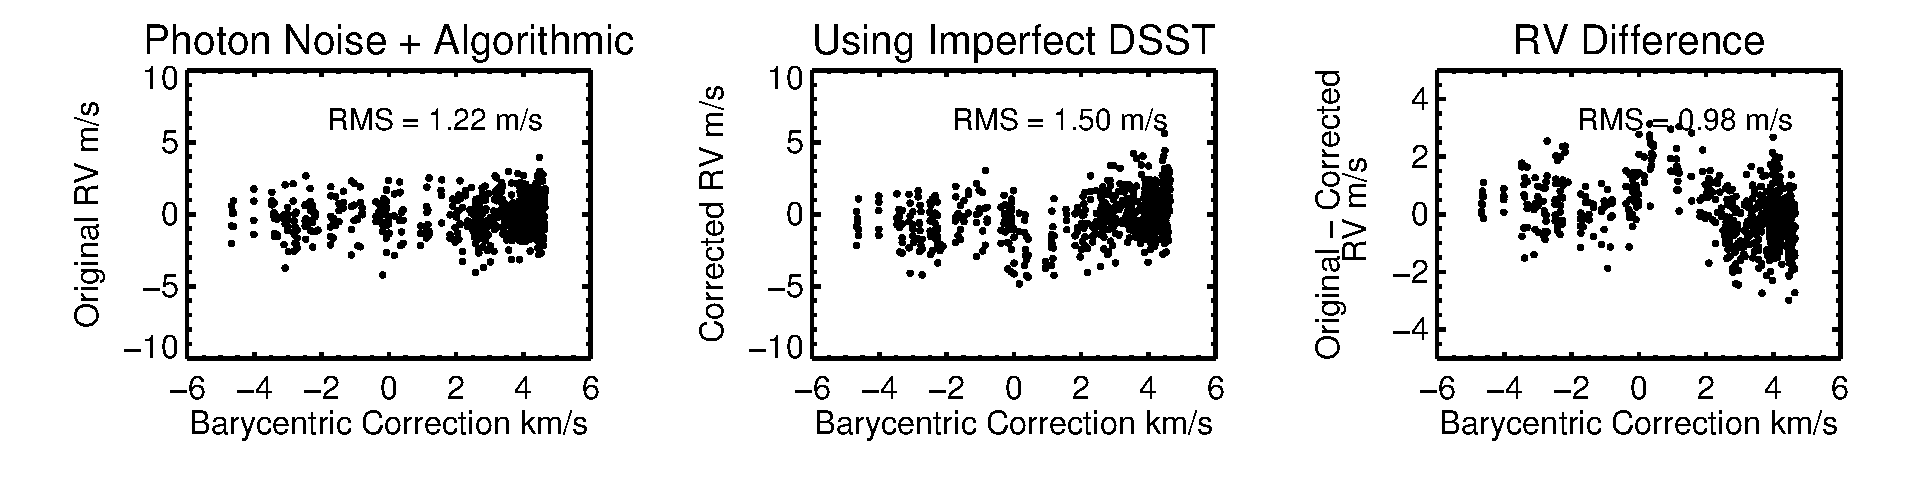
\includegraphics[scale=0.42]{keck/185144-rv-bc-3panel-test0-testd0.eps}}\
\subfloat[HD 10700]{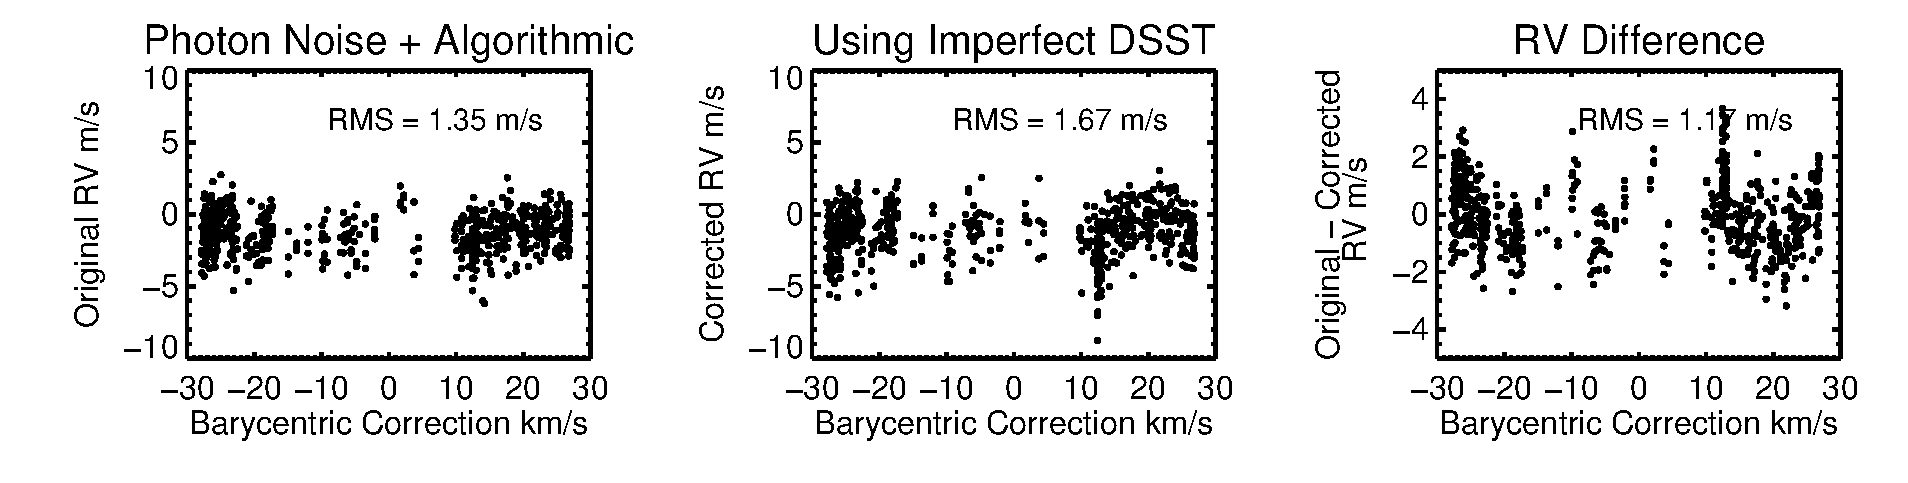
\includegraphics[scale=0.42]{keck/10700-rv-bc-3panel-test0-testd0.eps}}\
\caption{Effect of imperfect DSST on simulated data.
\label{keck:fig:dsst}}
\end{figure}
%----------------------------------------------------------------


%----------------------------------------------------------------
% Chunk illustration of effect of imperfect DSST
% plot made by ~/Exo.../Keck.../simulate.../msplot.pro, plot_name='makefakedsst','chunkcomp'
\begin{figure}
\subfloat{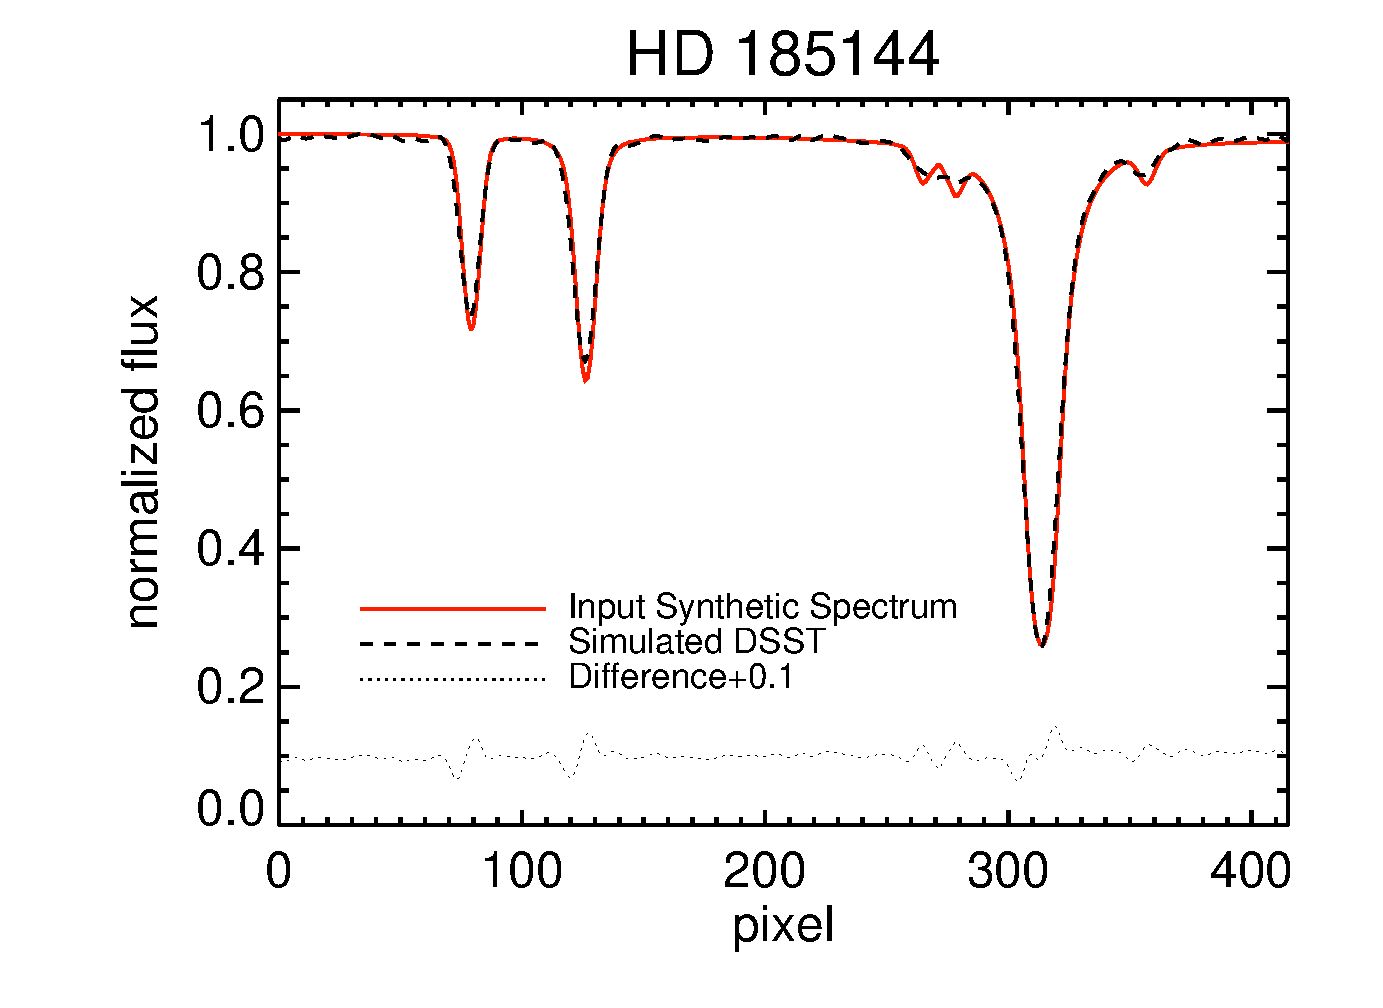
\includegraphics[scale=0.3]{keck/185144_makefakedsst_100.eps}}
\subfloat{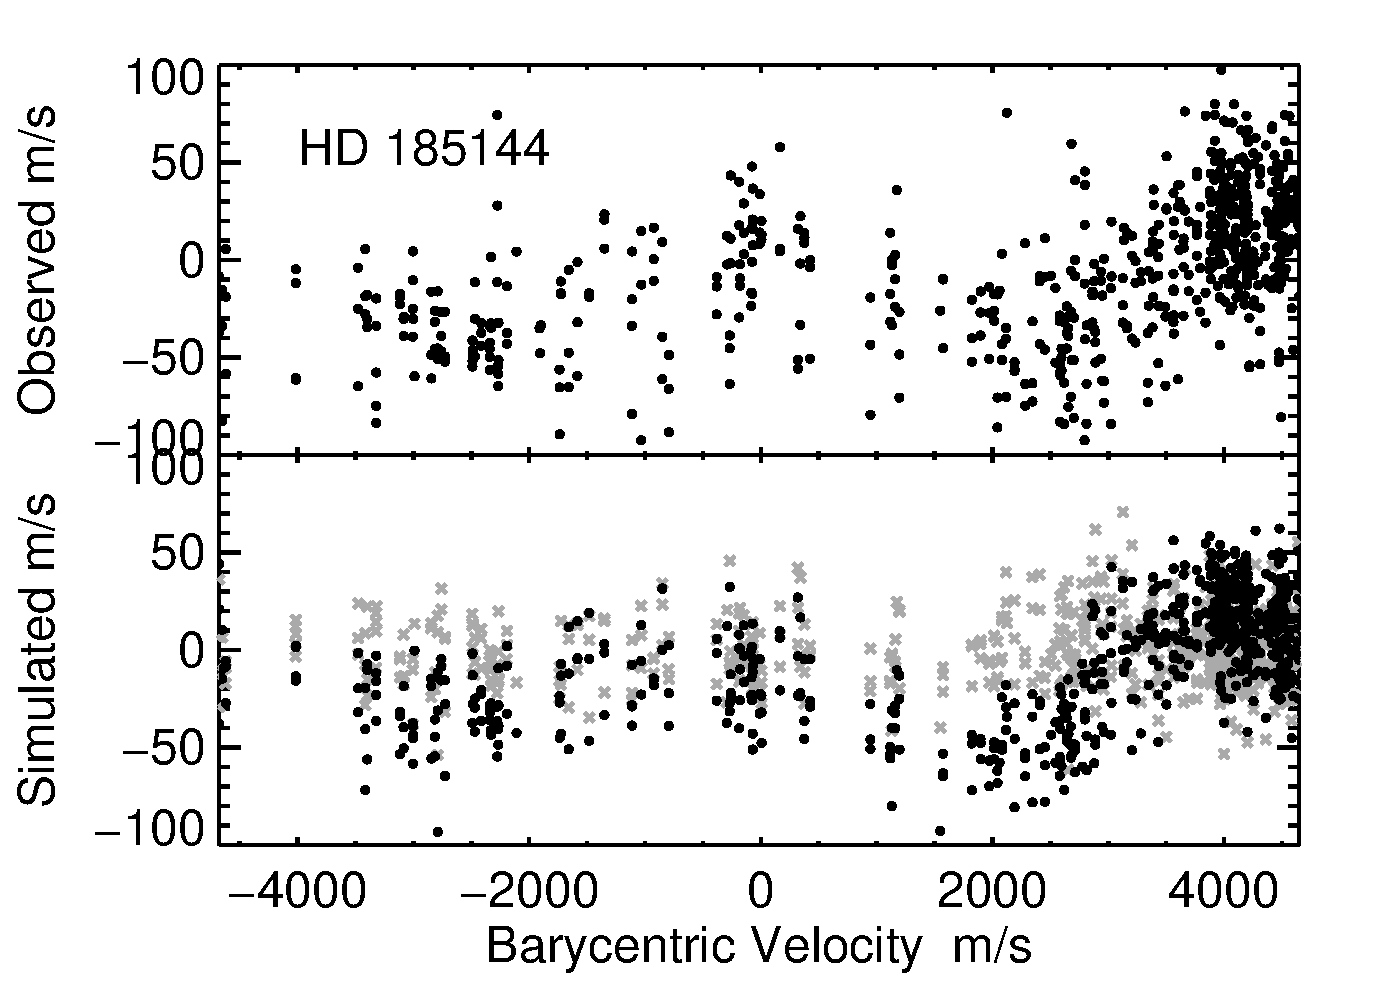
\includegraphics[scale=0.3]{keck/185144_chunkcomp_100.eps}}\
\subfloat{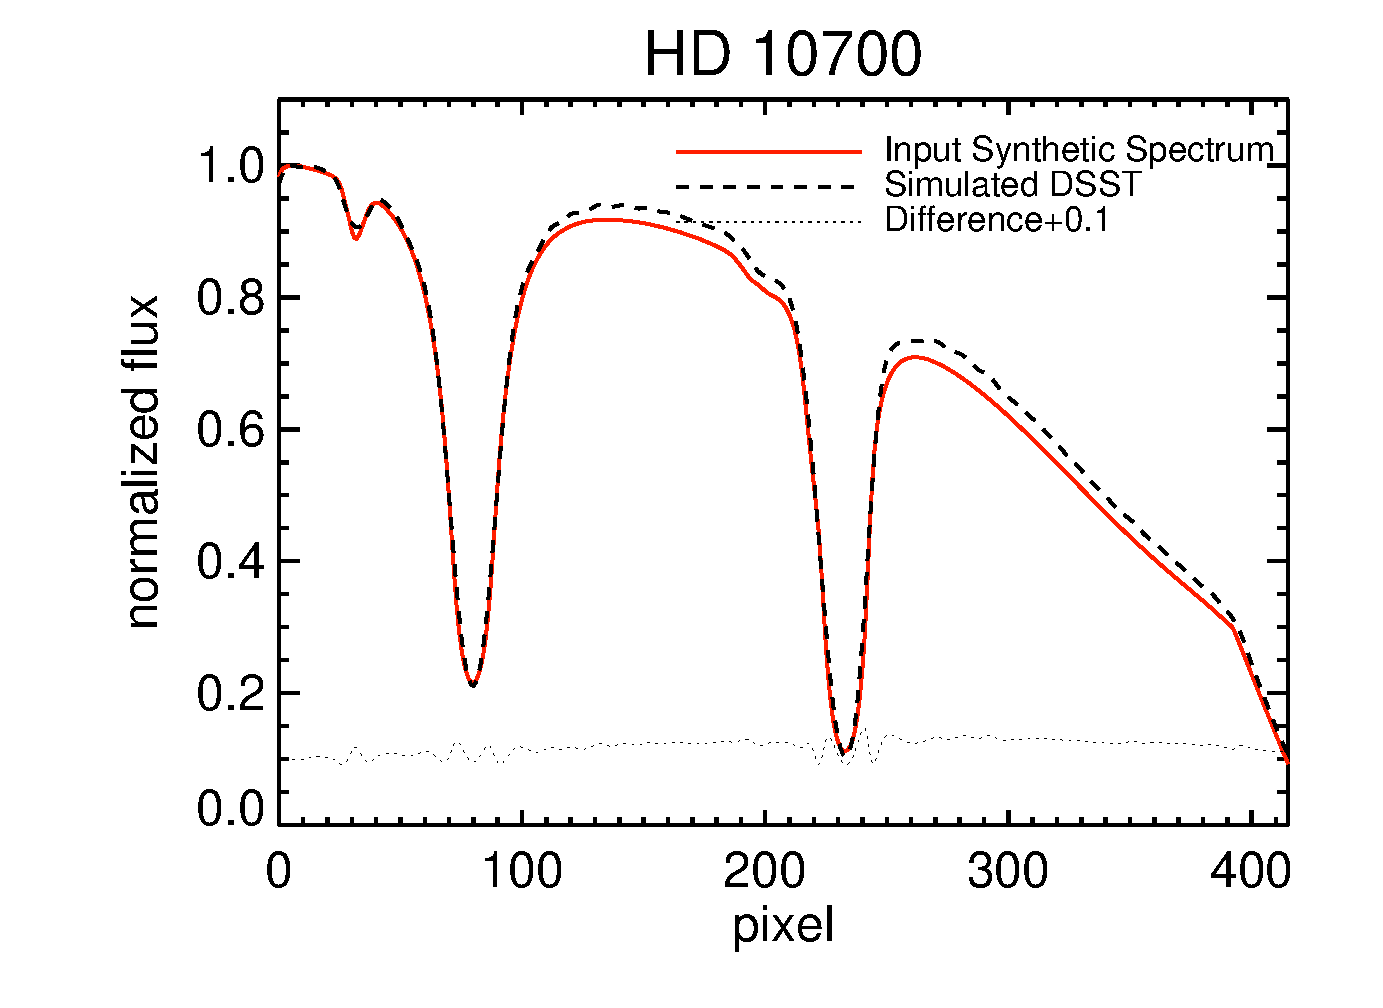
\includegraphics[scale=0.3]{keck/10700_makefakedsst_104.eps}}
\subfloat{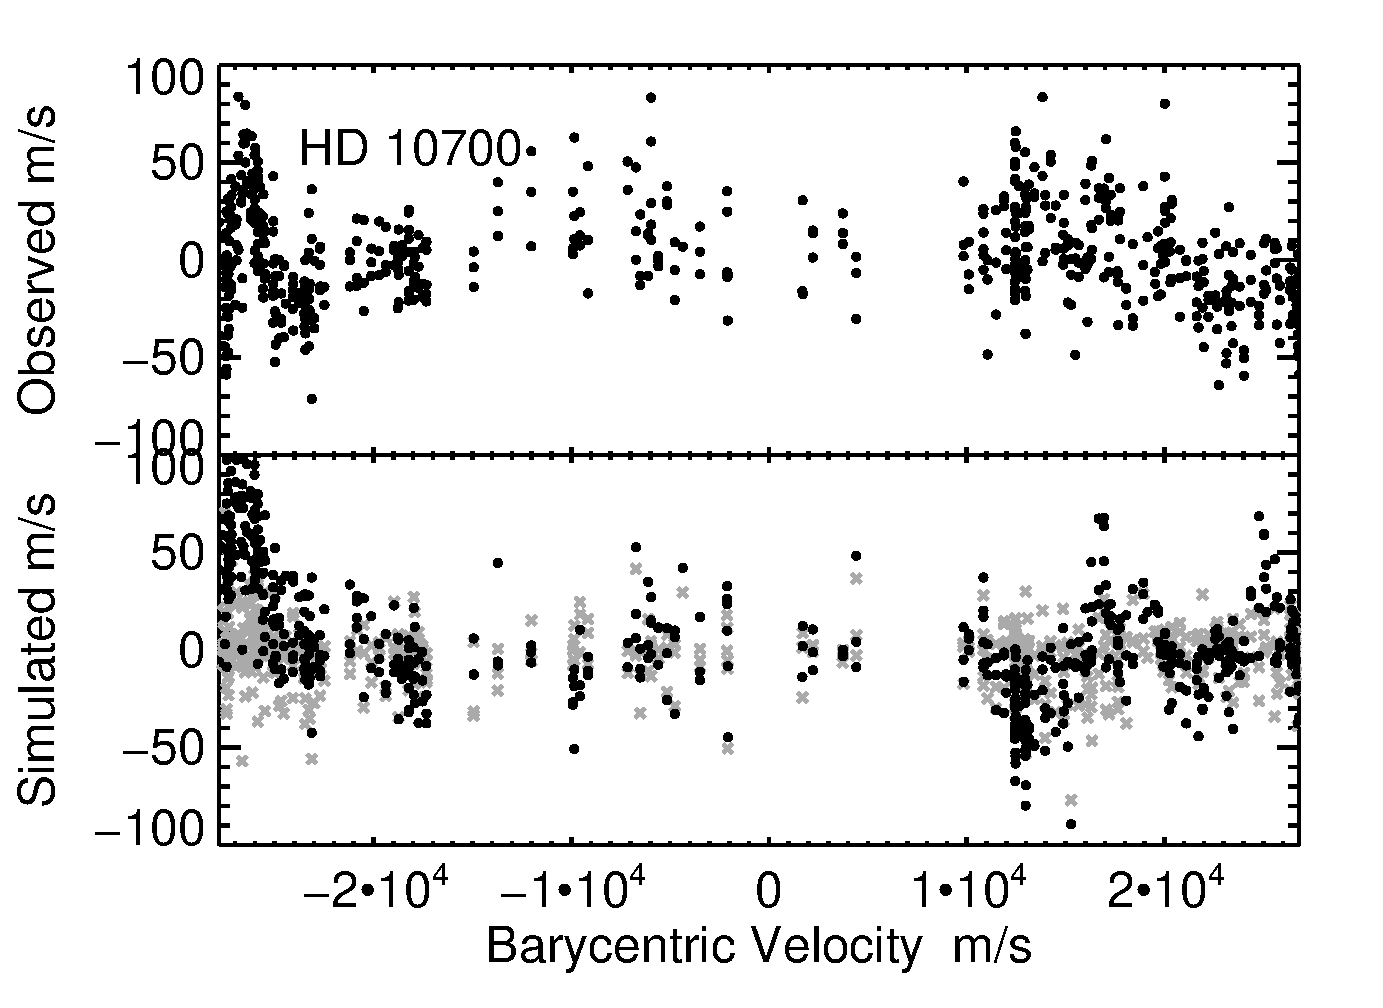
\includegraphics[scale=0.3]{keck/10700_chunkcomp_104.eps}}\
\caption{Effect of imperfect DSST on simulated data for a single
spectral chunk. HD 185144 is for a chunk near 5160\AA, and HD 10700 is
for a chunk around 5166\AA, which are spectral regions that tend to
receive high weights due to ample stellar lines and a lack of telluric
lines.
\label{keck:fig:dsstchunk}}
\end{figure}
%----------------------------------------------------------------

